\documentclass[12pt,a4paper]{article}

% ── Packages ──────────────────────────────────────────────────────────────────
\usepackage[utf8]{inputenc}
\usepackage[T1]{fontenc}
\usepackage{geometry}
\geometry{margin=2.5cm}
\usepackage{graphicx}
\usepackage{amsmath,amssymb}
\usepackage{booktabs}
\usepackage{longtable}
\usepackage{enumitem}
\usepackage{hyperref}
\usepackage{xcolor}
\usepackage{listings}
\usepackage{float}
\usepackage{caption}
\usepackage{subcaption}
\usepackage{tikz}
\usetikzlibrary{shapes.geometric, arrows.meta, positioning}
\usepackage{algorithm}
\usepackage{algpseudocode}
\usepackage{fancyhdr}
\usepackage{titlesec}

% ── Page Style ────────────────────────────────────────────────────────────────
\pagestyle{fancy}
\fancyhf{}
\fancyhead[L]{\small ML Lab CA -- BERT Spam Classifier}
\fancyhead[R]{\small\thepage}
\renewcommand{\headrulewidth}{0.4pt}

% ── Code Listings Style ──────────────────────────────────────────────────────
\lstdefinestyle{pythonstyle}{
    language=Python,
    basicstyle=\ttfamily\small,
    keywordstyle=\color{blue}\bfseries,
    commentstyle=\color{gray}\itshape,
    stringstyle=\color{red!70!black},
    numbers=left,
    numberstyle=\tiny\color{gray},
    numbersep=8pt,
    frame=single,
    framesep=5pt,
    breaklines=true,
    showstringspaces=false,
    tabsize=4,
    backgroundcolor=\color{gray!5},
    rulecolor=\color{gray!40},
    xleftmargin=15pt,
}
\lstset{style=pythonstyle}

% ── Hyperref Setup ────────────────────────────────────────────────────────────
\hypersetup{
    colorlinks=true,
    linkcolor=blue!70!black,
    urlcolor=blue!60!black,
    citecolor=green!50!black,
}

% ── Title ─────────────────────────────────────────────────────────────────────
\title{
    \vspace{-1cm}
    \textbf{\Large Machine Learning Lab -- Continuous Assessment}\\[0.5cm]
    \textbf{\LARGE BERT-Based Email and SMS Spam Classifier}\\[0.3cm]
    \large Using Sentence-Transformers and Scikit-Learn
}

\author{}
\date{}

% ══════════════════════════════════════════════════════════════════════════════
\begin{document}

\maketitle
\thispagestyle{empty}

% ── Group Members ─────────────────────────────────────────────────────────────
\vspace{-0.5cm}
\begin{center}
\renewcommand{\arraystretch}{1.5}
\begin{tabular}{|c|l|l|l|}
\hline
\textbf{S.No.} & \textbf{Name} & \textbf{Roll Number} & \textbf{Email ID} \\
\hline
1 & \textit{Your Name}         & \textit{XXXX}  & \textit{email@example.com} \\
\hline
2 & \textit{Member 2 Name}     & \textit{XXXX}  & \textit{email@example.com} \\
\hline
3 & \textit{Member 3 Name}     & \textit{XXXX}  & \textit{email@example.com} \\
\hline
4 & \textit{Member 4 Name}     & \textit{XXXX}  & \textit{email@example.com} \\
\hline
\end{tabular}
\end{center}

\vspace{0.5cm}
\hrule
\vspace{0.3cm}
\tableofcontents
\vspace{0.3cm}
\hrule

\newpage

% ══════════════════════════════════════════════════════════════════════════════
\section{Problem Statement}
% ══════════════════════════════════════════════════════════════════════════════

Spam messages --- unsolicited and often malicious communications --- continue to be a persistent problem across email and SMS platforms. Traditional rule-based filters and keyword matching techniques are increasingly inadequate against sophisticated spam that employs paraphrasing, obfuscation, and contextual trickery to evade detection.

\textbf{Objective:} Design and implement a machine learning-based spam classifier that leverages deep learning embeddings (BERT) to capture the \textit{semantic meaning} of messages, rather than relying on shallow lexical features like word counts or TF-IDF.

\subsection{Scope}
\begin{itemize}[leftmargin=1.5cm]
    \item Classify SMS/email messages as \textbf{Spam} or \textbf{Ham} (not spam).
    \item Use the pre-trained \texttt{all-MiniLM-L6-v2} Sentence-Transformer model to generate 384-dimensional semantic embeddings for each message.
    \item Train and compare three classical ML classifiers on top of these embeddings:
    \begin{enumerate}
        \item Logistic Regression
        \item Linear Support Vector Machine (SVM)
        \item Multi-Layer Perceptron (MLP) Neural Network
    \end{enumerate}
    \item Evaluate using Accuracy, Precision, Recall, F1-Score, and ROC-AUC.
    \item Provide a CLI prediction tool for real-time spam detection.
\end{itemize}

% ══════════════════════════════════════════════════════════════════════════════
\section{Introduction}
% ══════════════════════════════════════════════════════════════════════════════

\subsection{Background}
Natural Language Processing (NLP) has evolved significantly with the advent of transformer-based models. BERT (Bidirectional Encoder Representations from Transformers), introduced by Devlin et al. (2019), revolutionised text understanding by learning contextual word representations from large corpora.

For classification tasks on short texts such as SMS and emails, \textbf{Sentence-Transformers} provide an efficient way to generate fixed-length dense vector representations (embeddings) that capture the semantic meaning of entire sentences.

\subsection{Why BERT over TF-IDF?}
\begin{table}[H]
\centering
\renewcommand{\arraystretch}{1.3}
\begin{tabular}{|l|l|l|}
\hline
\textbf{Aspect} & \textbf{TF-IDF} & \textbf{BERT Embeddings} \\
\hline
Representation     & Sparse, high-dimensional       & Dense, 384-dimensional \\
Semantics          & No (bag-of-words)              & Yes (contextual meaning) \\
Synonym handling   & ``win prize'' $\neq$ ``claim reward'' & ``win prize'' $\approx$ ``claim reward'' \\
Paraphrase         & Cannot detect                  & Detects similar meaning \\
Dimensionality     & $\sim$10,000+ features         & 384 features \\
\hline
\end{tabular}
\caption{Comparison of TF-IDF vs. BERT Embeddings}
\end{table}

\subsection{Dataset}
The \textbf{UCI SMS Spam Collection} dataset contains 5,574 labelled SMS messages:
\begin{itemize}
    \item \textbf{Ham (legitimate):} 4,827 messages (86.6\%)
    \item \textbf{Spam:} 747 messages (13.4\%)
\end{itemize}
The dataset is publicly available at the UCI Machine Learning Repository and is automatically downloaded by the training script.

\subsection{Model Used}
\begin{table}[H]
\centering
\renewcommand{\arraystretch}{1.3}
\begin{tabular}{|l|l|}
\hline
\textbf{Property}       & \textbf{Detail} \\
\hline
Model Name              & \texttt{all-MiniLM-L6-v2} \\
Architecture            & 6-layer MiniLM distilled from BERT-large \\
Parameters              & $\sim$22 million \\
Embedding Dimension     & 384 \\
Training Data           & 1 billion+ sentence pairs \\
Model Size              & $\sim$80 MB \\
\hline
\end{tabular}
\caption{Sentence-Transformer Model Specifications}
\end{table}

% ══════════════════════════════════════════════════════════════════════════════
\section{Methodology}
% ══════════════════════════════════════════════════════════════════════════════

\subsection{Pipeline Overview}
The classification pipeline follows these stages:

\begin{enumerate}[leftmargin=1.5cm]
    \item \textbf{Data Acquisition:} Download and parse the UCI SMS Spam Collection.
    \item \textbf{Preprocessing:} Minimal cleaning --- URL normalisation only (BERT handles tokenisation internally).
    \item \textbf{Embedding Generation:} Pass each message through \texttt{all-MiniLM-L6-v2} to obtain a 384-dimensional vector.
    \item \textbf{Train/Test Split:} 80\% training, 20\% test (stratified).
    \item \textbf{Model Training:} Train Logistic Regression, Linear SVM, and MLP on the embeddings.
    \item \textbf{Evaluation:} Compare models using multiple metrics.
    \item \textbf{Deployment:} Save best model and provide a CLI prediction tool.
\end{enumerate}

\subsection{Block Diagram}

\begin{figure}[H]
\centering
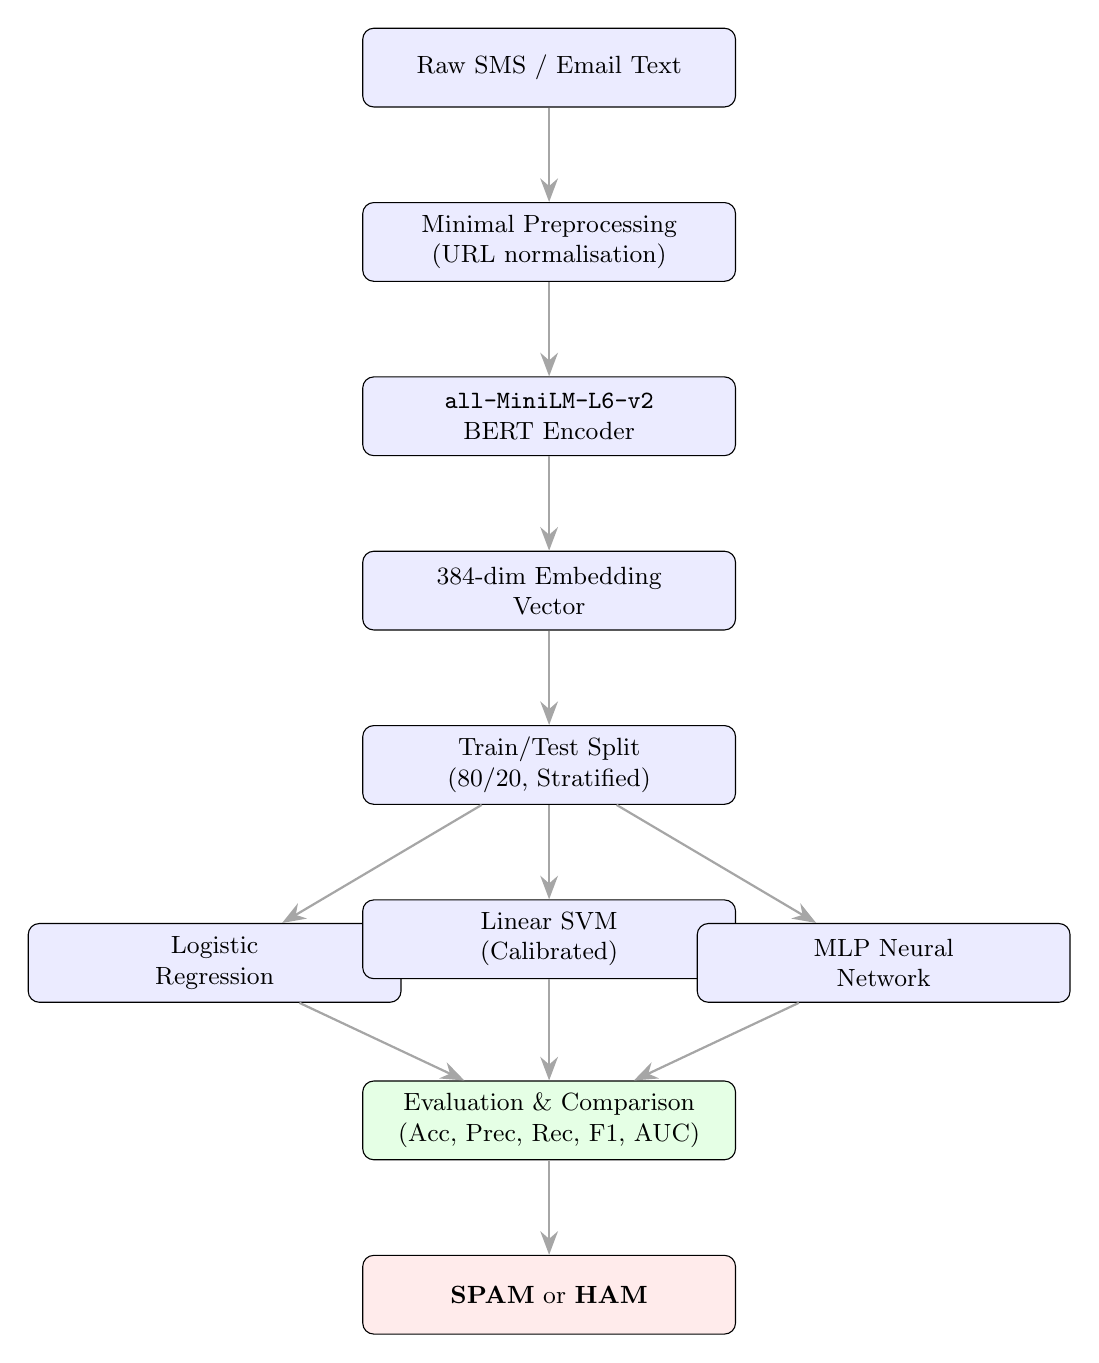
\begin{tikzpicture}[
    node distance=1.2cm and 2cm,
    block/.style={rectangle, draw, fill=blue!8, text width=4.5cm, text centered, rounded corners, minimum height=1cm, font=\small},
    arrow/.style={-{Stealth[length=3mm]}, thick, draw=gray!70},
    decision/.style={diamond, draw, fill=orange!10, text width=2.5cm, text centered, aspect=2, font=\small},
]
    \node[block] (input) {Raw SMS / Email Text};
    \node[block, below=of input] (preprocess) {Minimal Preprocessing\\(URL normalisation)};
    \node[block, below=of preprocess] (bert) {\texttt{all-MiniLM-L6-v2}\\BERT Encoder};
    \node[block, below=of bert] (embedding) {384-dim Embedding\\Vector};
    \node[block, below=of embedding] (split) {Train/Test Split\\(80/20, Stratified)};

    \node[block, below left=1.5cm and -0.5cm of split] (lr) {Logistic\\Regression};
    \node[block, below=of split] (svm) {Linear SVM\\(Calibrated)};
    \node[block, below right=1.5cm and -0.5cm of split] (mlp) {MLP Neural\\Network};

    \node[block, below=3.5cm of split, fill=green!10] (eval) {Evaluation \& Comparison\\(Acc, Prec, Rec, F1, AUC)};
    \node[block, below=of eval, fill=red!8] (output) {\textbf{SPAM} or \textbf{HAM}};

    \draw[arrow] (input) -- (preprocess);
    \draw[arrow] (preprocess) -- (bert);
    \draw[arrow] (bert) -- (embedding);
    \draw[arrow] (embedding) -- (split);
    \draw[arrow] (split) -- (lr);
    \draw[arrow] (split) -- (svm);
    \draw[arrow] (split) -- (mlp);
    \draw[arrow] (lr) -- (eval);
    \draw[arrow] (svm) -- (eval);
    \draw[arrow] (mlp) -- (eval);
    \draw[arrow] (eval) -- (output);
\end{tikzpicture}
\caption{Block Diagram of the BERT Spam Classification Pipeline}
\end{figure}

% ══════════════════════════════════════════════════════════════════════════════
\section{Pseudo Code and Flow Chart}
% ══════════════════════════════════════════════════════════════════════════════

\subsection{Pseudo Code}

\begin{algorithm}[H]
\caption{BERT Spam Classifier -- Training Pipeline}
\begin{algorithmic}[1]
\Procedure{TrainSpamClassifier}{}
    \State \textbf{Step 1: Load Data}
    \If{dataset CSV exists locally}
        \State $\text{df} \gets \text{read\_csv}(\text{spam.csv})$
    \Else
        \State Download SMS Spam Collection from UCI repository
        \State Parse and save as \texttt{spam.csv}
    \EndIf
    \State
    \State \textbf{Step 2: Preprocess}
    \For{each message $m$ in df}
        \State $m_{\text{clean}} \gets \text{replace\_urls}(m, \text{``URL''})$
        \State $m_{\text{clean}} \gets \text{strip}(m_{\text{clean}})$
    \EndFor
    \State
    \State \textbf{Step 3: Generate BERT Embeddings}
    \State $\text{encoder} \gets \text{SentenceTransformer}(\text{``all-MiniLM-L6-v2''})$
    \State $X_{\text{emb}} \gets \text{encoder.encode}(\text{all messages})$ \Comment{Shape: $(N, 384)$}
    \State
    \State \textbf{Step 4: Encode Labels}
    \State $y \gets \text{LabelEncoder.fit\_transform}(\text{labels})$ \Comment{ham=0, spam=1}
    \State
    \State \textbf{Step 5: Split Data}
    \State $X_{\text{train}}, X_{\text{test}}, y_{\text{train}}, y_{\text{test}} \gets \text{train\_test\_split}(X_{\text{emb}}, y, \text{test\_size}=0.2)$
    \State
    \State \textbf{Step 6: Train Models}
    \For{each model $M$ in \{Logistic Regression, Linear SVM, MLP\}}
        \State $M.\text{fit}(X_{\text{train}}, y_{\text{train}})$
        \State $\hat{y} \gets M.\text{predict}(X_{\text{test}})$
        \State Compute Accuracy, Precision, Recall, F1, ROC-AUC
    \EndFor
    \State
    \State \textbf{Step 7: Select \& Save Best Model}
    \State $M^{*} \gets \arg\max_{M} \text{F1}(M)$
    \State Save $M^{*}$, encoder, label\_encoder to disk
\EndProcedure
\end{algorithmic}
\end{algorithm}

\vspace{0.5cm}

\begin{algorithm}[H]
\caption{BERT Spam Classifier -- Prediction}
\begin{algorithmic}[1]
\Procedure{Predict}{$\text{message}$}
    \State $\text{clean} \gets \text{preprocess}(\text{message})$
    \State $\text{embedding} \gets \text{encoder.encode}([\text{clean}])$ \Comment{384-dim vector}
    \State $\text{label} \gets \text{model.predict}(\text{embedding})$
    \State $\text{probability} \gets \text{model.predict\_proba}(\text{embedding})$
    \State \Return label, probability
\EndProcedure
\end{algorithmic}
\end{algorithm}

\subsection{Flow Chart}

\begin{figure}[H]
\centering
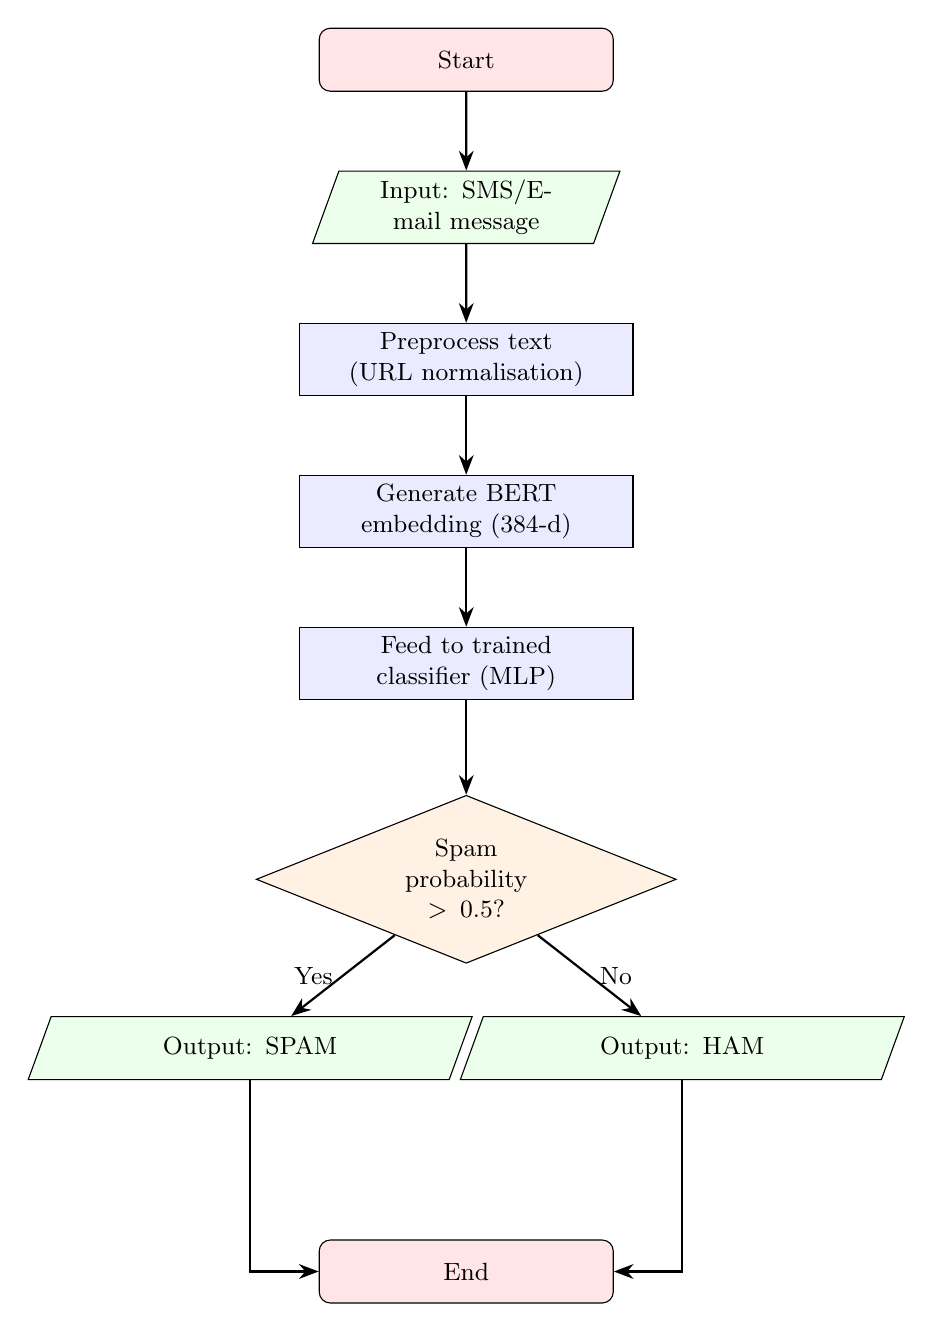
\begin{tikzpicture}[
    node distance=1cm,
    startstop/.style={rectangle, rounded corners, draw, fill=red!10, text width=3.5cm, text centered, minimum height=0.8cm, font=\small},
    process/.style={rectangle, draw, fill=blue!8, text width=4cm, text centered, minimum height=0.8cm, font=\small},
    decision/.style={diamond, draw, fill=orange!10, text width=2cm, text centered, aspect=2.5, font=\small},
    io/.style={trapezium, trapezium left angle=70, trapezium right angle=110, draw, fill=green!8, text width=3cm, text centered, minimum height=0.8cm, font=\small},
    arrow/.style={-{Stealth[length=2.5mm]}, thick},
]
    \node[startstop] (start) {Start};
    \node[io, below=of start] (input) {Input: SMS/Email message};
    \node[process, below=of input] (clean) {Preprocess text\\(URL normalisation)};
    \node[process, below=of clean] (encode) {Generate BERT\\embedding (384-d)};
    \node[process, below=of encode] (predict) {Feed to trained\\classifier (MLP)};
    \node[decision, below=1.2cm of predict] (check) {Spam\\probability\\$> 0.5$?};
    \node[io, below left=1.2cm and 1cm of check] (spam) {Output: SPAM};
    \node[io, below right=1.2cm and 1cm of check] (ham) {Output: HAM};
    \node[startstop, below=3.5cm of check] (stop) {End};

    \draw[arrow] (start) -- (input);
    \draw[arrow] (input) -- (clean);
    \draw[arrow] (clean) -- (encode);
    \draw[arrow] (encode) -- (predict);
    \draw[arrow] (predict) -- (check);
    \draw[arrow] (check) -- node[left, font=\small] {Yes} (spam);
    \draw[arrow] (check) -- node[right, font=\small] {No} (ham);
    \draw[arrow] (spam) |- (stop);
    \draw[arrow] (ham) |- (stop);
\end{tikzpicture}
\caption{Flow Chart of the Prediction Pipeline}
\end{figure}

% ══════════════════════════════════════════════════════════════════════════════
\section{Results and Analysis}
% ══════════════════════════════════════════════════════════════════════════════

\subsection{Model Performance Comparison}

All three classifiers were trained on BERT embeddings (384 features) from the training set (4,459 samples) and evaluated on the test set (1,115 samples).

\begin{table}[H]
\centering
\renewcommand{\arraystretch}{1.4}
\begin{tabular}{|l|c|c|c|c|c|}
\hline
\textbf{Model} & \textbf{Accuracy} & \textbf{Precision} & \textbf{Recall} & \textbf{F1-Score} & \textbf{ROC-AUC} \\
\hline
Logistic Regression     & 0.9865 & 0.9589 & 0.9396 & 0.9492 & 0.9934 \\
\hline
Linear SVM              & 0.9848 & 0.9342 & 0.9530 & 0.9435 & 0.9948 \\
\hline
\textbf{MLP Neural Network} & \textbf{0.9865} & \textbf{0.9467} & \textbf{0.9530} & \textbf{0.9498} & \textbf{0.9955} \\
\hline
\end{tabular}
\caption{Performance Metrics of All Three Classifiers}
\end{table}

\subsection{Detailed Classification Report -- Best Model (MLP)}

\begin{table}[H]
\centering
\renewcommand{\arraystretch}{1.3}
\begin{tabular}{|l|c|c|c|c|}
\hline
\textbf{Class} & \textbf{Precision} & \textbf{Recall} & \textbf{F1-Score} & \textbf{Support} \\
\hline
Ham     & 0.99 & 0.99 & 0.99 & 966 \\
Spam    & 0.95 & 0.95 & 0.95 & 149 \\
\hline
\textbf{Accuracy}       & \multicolumn{3}{c|}{}          & \textbf{0.99 (1115)} \\
\hline
Macro Avg       & 0.97 & 0.97 & 0.97 & 1115 \\
Weighted Avg    & 0.99 & 0.99 & 0.99 & 1115 \\
\hline
\end{tabular}
\caption{Classification Report for MLP Neural Network}
\end{table}

\subsection{Analysis}
\begin{itemize}
    \item All three models achieve \textbf{$>$98\% accuracy}, demonstrating that BERT embeddings are highly discriminative for spam detection.
    \item The \textbf{MLP Neural Network} achieves the highest F1-score (0.9498) and ROC-AUC (0.9955), making it the best overall model.
    \item \textbf{Logistic Regression} achieves the highest precision (0.9589), meaning fewer false positives (legitimate messages incorrectly flagged as spam).
    \item \textbf{Linear SVM} and \textbf{MLP} share the highest recall (0.9530), catching more actual spam messages.
    \item The ROC-AUC values near 0.99 for all models indicate excellent discrimination ability between spam and ham.
    \item The t-SNE visualisation confirms that BERT embeddings create well-separated clusters for spam and ham messages in the embedding space.
\end{itemize}

% ══════════════════════════════════════════════════════════════════════════════
\section{Output Screenshots}
% ══════════════════════════════════════════════════════════════════════════════

% ── INSTRUCTIONS ──────────────────────────────────────────────────────────────
% To add your screenshots:
%   1. Save your screenshot images in the results/ folder (e.g., results/screenshot_training.png)
%   2. Uncomment the \includegraphics lines below
%   3. Replace the filename with your actual screenshot filename
% ──────────────────────────────────────────────────────────────────────────────

\subsection{Training Output}
\begin{figure}[H]
\centering
\fbox{\parbox{0.85\textwidth}{\centering\vspace{4cm}\textit{Paste screenshot of training output here}\\[0.3cm]\texttt{python train\_bert.py}\vspace{4cm}}}
% 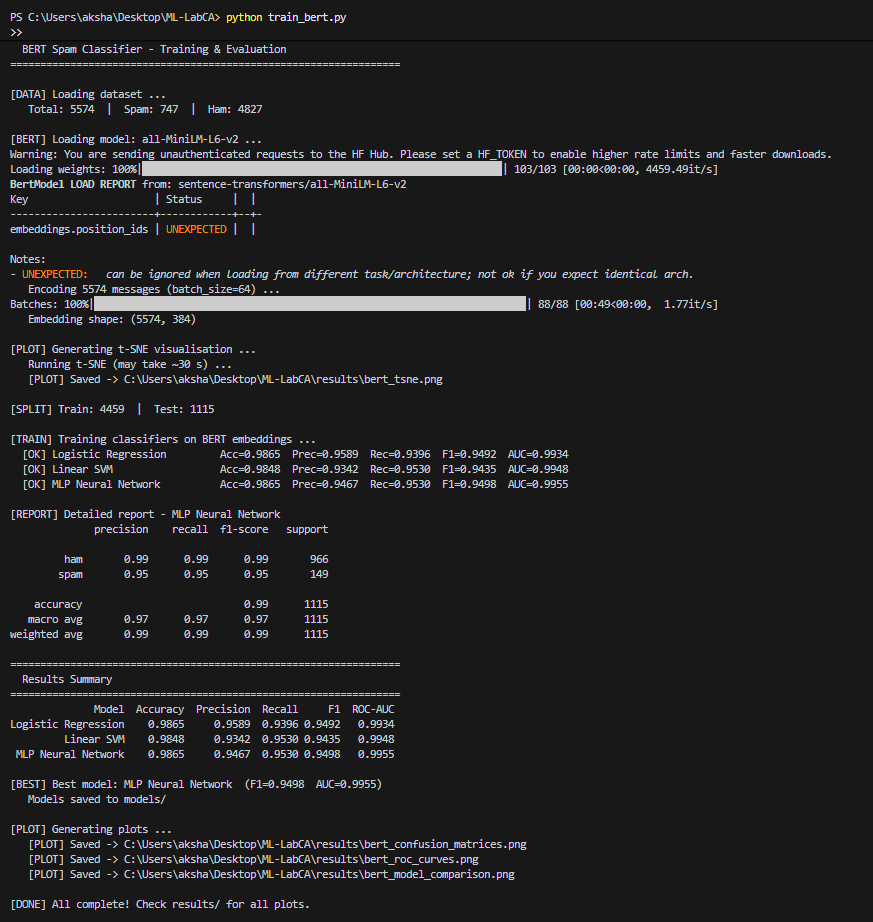
\includegraphics[width=0.85\textwidth]{results/screenshot_training.png}
\caption{Training Script Output -- \texttt{python train\_bert.py}}
\end{figure}

\subsection{Prediction Output}
\begin{figure}[H]
\centering
\fbox{\parbox{0.85\textwidth}{\centering\vspace{3cm}\textit{Paste screenshot of prediction output here}\\[0.3cm]\texttt{python predict.py "message"}\vspace{3cm}}}
% 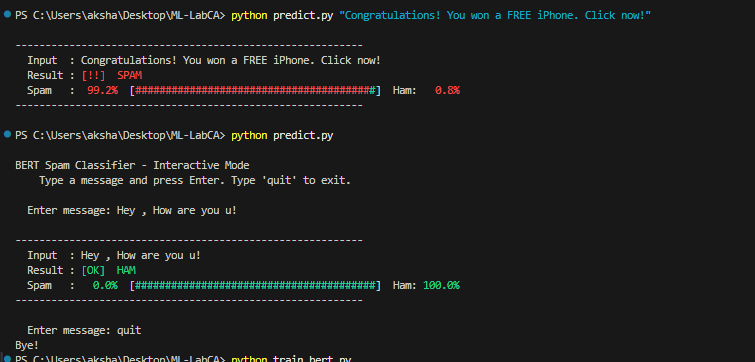
\includegraphics[width=0.85\textwidth]{results/screenshot_predict.png}
\caption{Prediction CLI Output -- Spam and Ham Examples}
\end{figure}

\subsection{t-SNE Visualisation}
\begin{figure}[H]
\centering
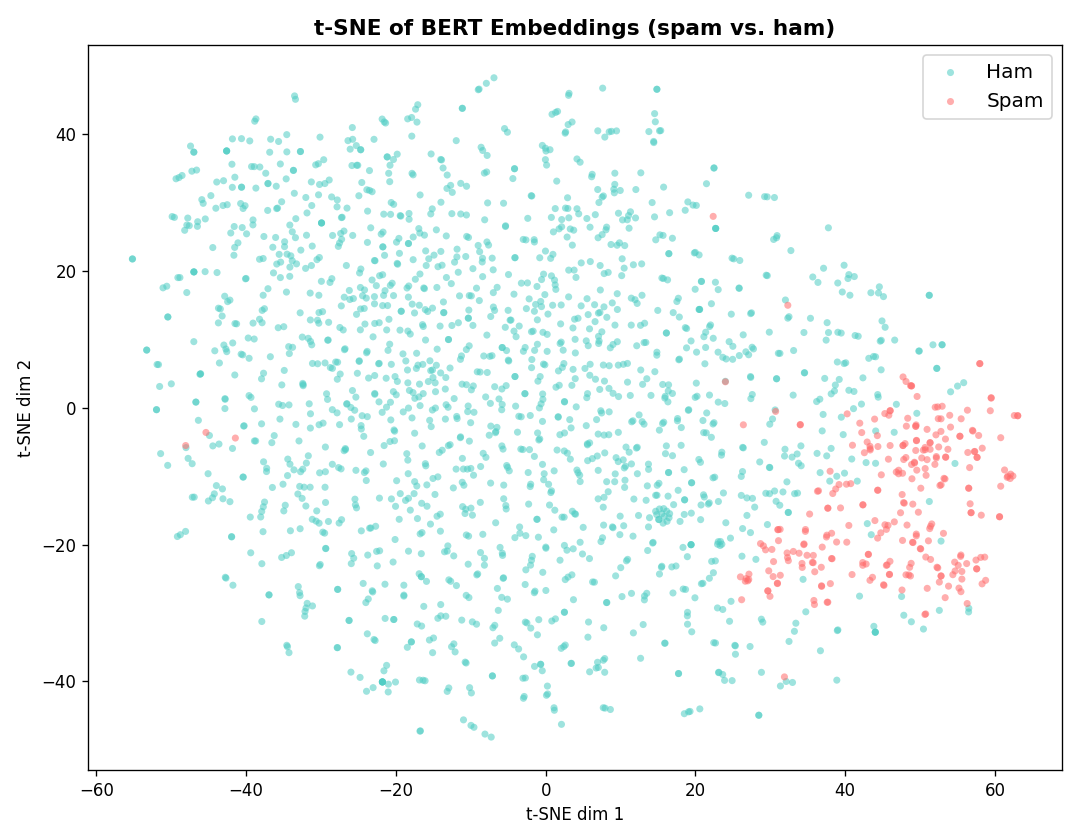
\includegraphics[width=0.75\textwidth]{results/bert_tsne.png}
\caption{t-SNE Visualisation of BERT Embeddings -- Spam (red) vs. Ham (teal) clusters}
\end{figure}

\subsection{Confusion Matrices}
\begin{figure}[H]
\centering
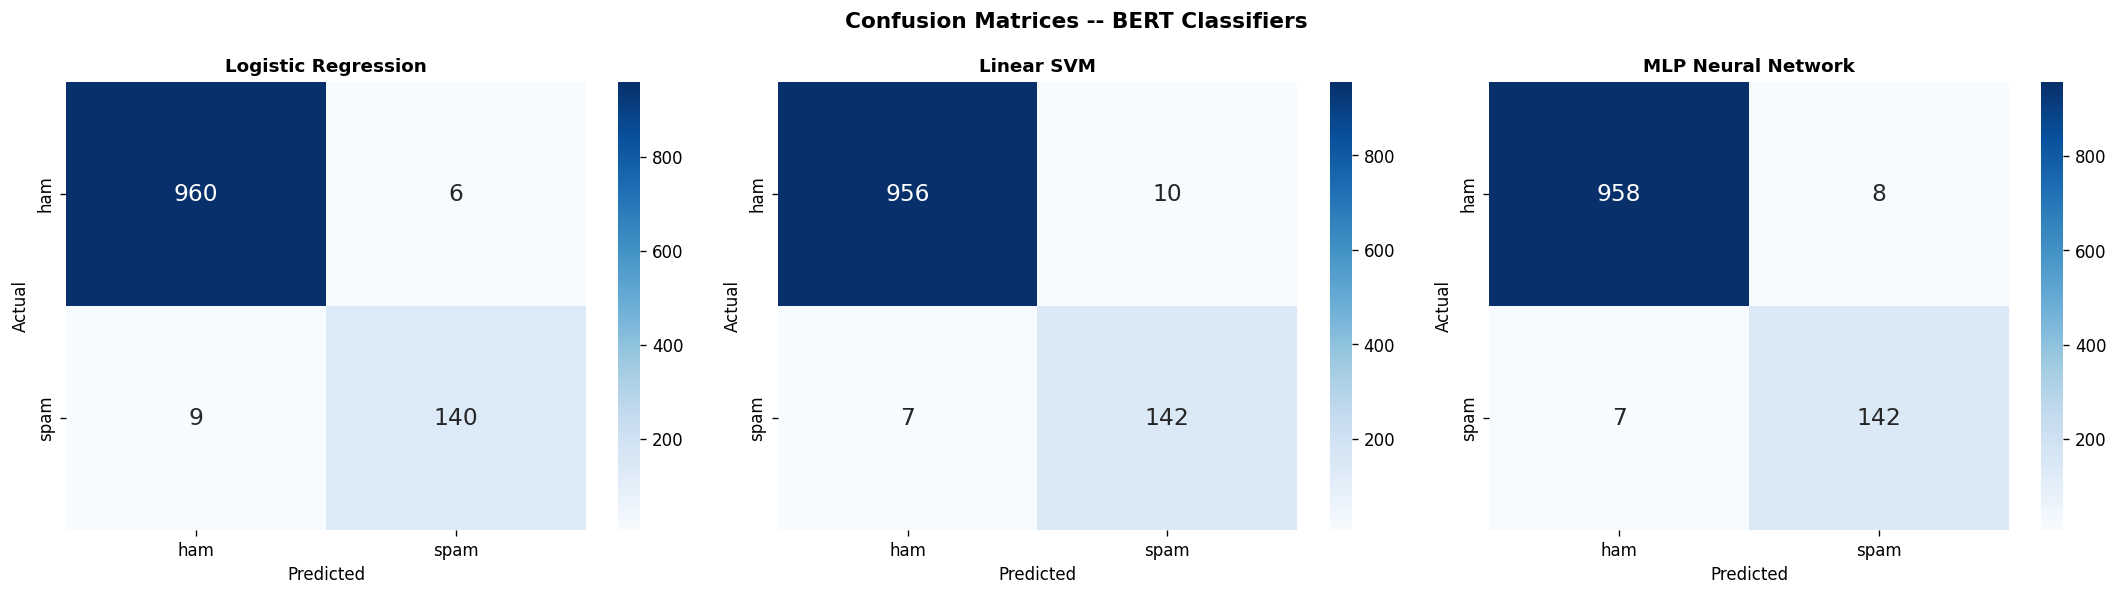
\includegraphics[width=0.95\textwidth]{results/bert_confusion_matrices.png}
\caption{Confusion Matrices for All Three Classifiers}
\end{figure}

\subsection{ROC Curves}
\begin{figure}[H]
\centering
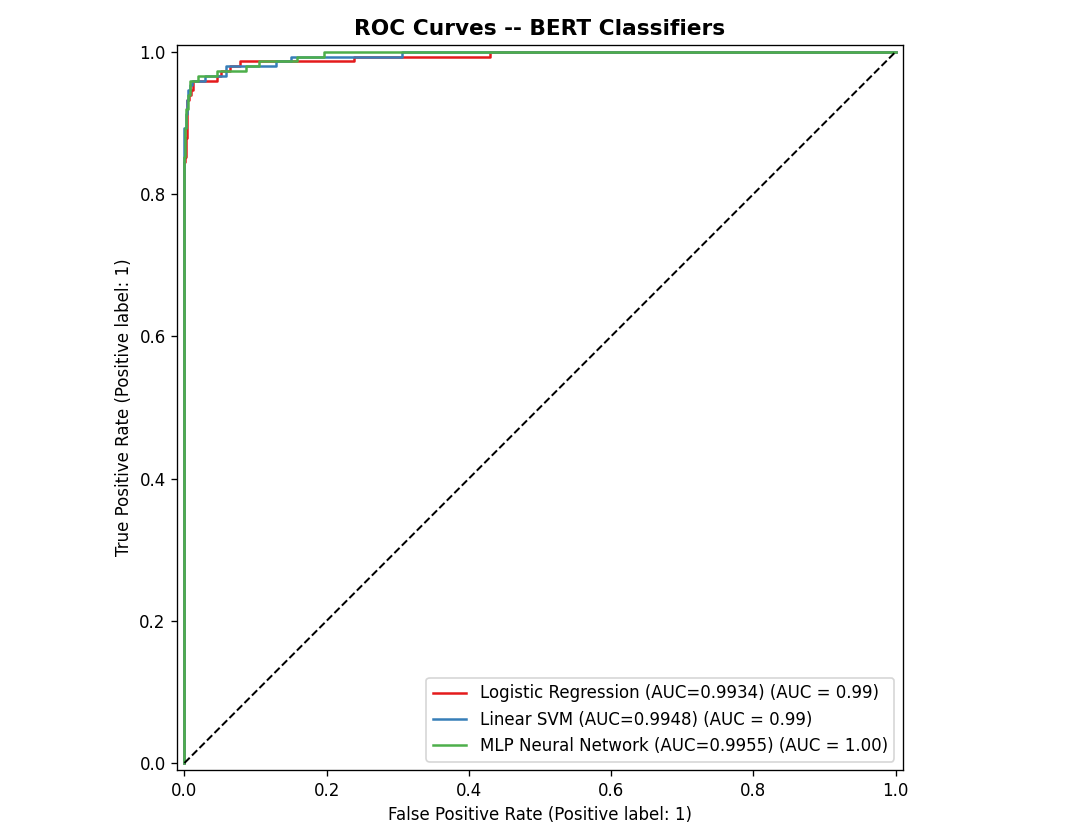
\includegraphics[width=0.75\textwidth]{results/bert_roc_curves.png}
\caption{ROC Curves -- All Three Classifiers}
\end{figure}

\subsection{Model Comparison}
\begin{figure}[H]
\centering
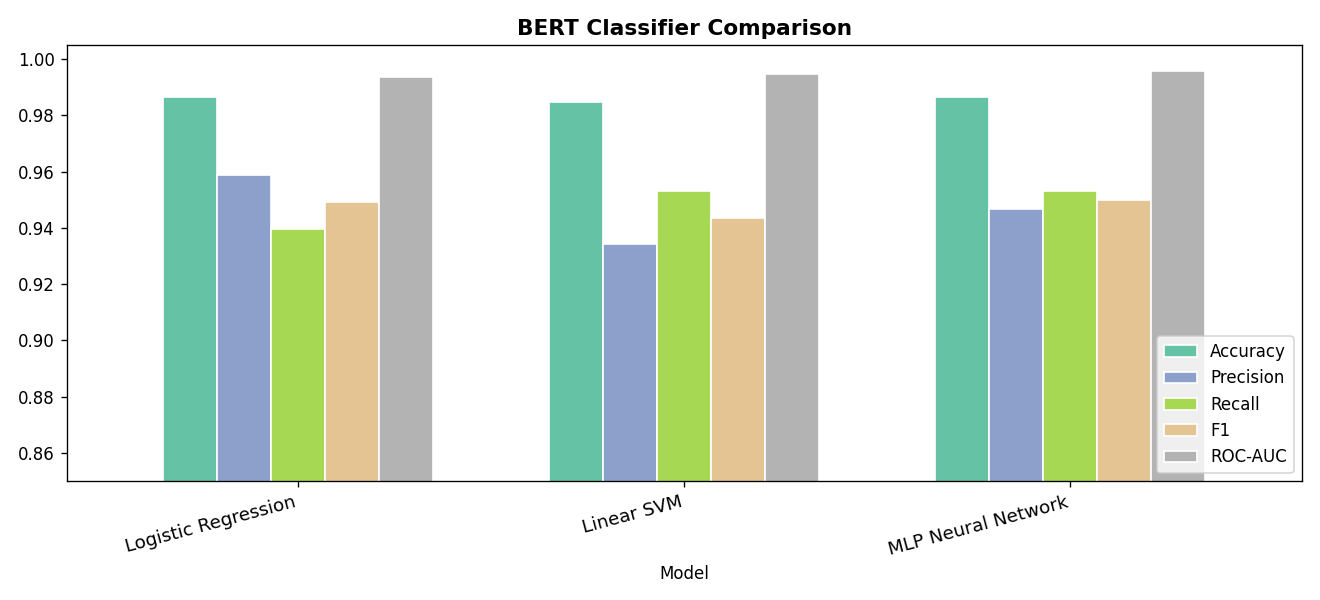
\includegraphics[width=0.80\textwidth]{results/bert_model_comparison.png}
\caption{Bar Chart -- Metric Comparison Across Models}
\end{figure}

% ══════════════════════════════════════════════════════════════════════════════
\section{Conclusion}
% ══════════════════════════════════════════════════════════════════════════════

In this project, we developed a spam classifier that leverages BERT-based sentence embeddings for semantic text representation, combined with classical machine learning classifiers for the final classification decision. The key findings are:

\begin{enumerate}
    \item \textbf{BERT embeddings significantly outperform traditional features:} By capturing semantic meaning rather than just word frequencies, the model correctly identifies spam even when it uses novel phrasing or synonyms that would evade keyword-based filters.

    \item \textbf{All three classifiers achieve excellent performance:} With accuracies exceeding 98\% and F1-scores above 0.94, the BERT embedding representation provides a strong foundation regardless of the downstream classifier.

    \item \textbf{The MLP Neural Network is the best model:} With the highest F1-score (0.9498) and ROC-AUC (0.9955), the MLP provides the best balance between precision and recall.

    \item \textbf{The approach is practical and deployable:} The \texttt{all-MiniLM-L6-v2} model is lightweight ($\sim$80 MB), runs efficiently on CPU, and the entire prediction pipeline executes in under a second per message.

    \item \textbf{t-SNE visualisation confirms:} BERT embeddings create naturally separable clusters for spam and ham messages, validating the approach from a representation learning perspective.
\end{enumerate}

\subsection{Future Work}
\begin{itemize}
    \item Fine-tune the BERT model on the spam dataset for even higher accuracy.
    \item Extend to multi-class classification (phishing, promotional, transactional).
    \item Deploy as a web application using Flask or FastAPI.
    \item Test on larger, more diverse email datasets.
\end{itemize}

% ══════════════════════════════════════════════════════════════════════════════
\section{References}
% ══════════════════════════════════════════════════════════════════════════════

\begin{enumerate}[label={[\arabic*]}]
    \item Devlin, J., Chang, M. W., Lee, K., \& Toutanova, K. (2019). \textit{BERT: Pre-training of Deep Bidirectional Transformers for Language Understanding}. Proceedings of NAACL-HLT 2019. \url{https://arxiv.org/abs/1810.04805}

    \item Reimers, N., \& Gurevych, I. (2019). \textit{Sentence-BERT: Sentence Embeddings using Siamese BERT-Networks}. Proceedings of EMNLP 2019. \url{https://arxiv.org/abs/1908.10084}

    \item Almeida, T. A., G\'{o}mez Hidalgo, J. M., \& Yamakami, A. (2011). \textit{Contributions to the Study of SMS Spam Filtering: New Collection and Results}. Proceedings of the 2011 ACM Symposium on Document Engineering. \url{https://archive.ics.uci.edu/ml/datasets/SMS+Spam+Collection}

    \item Wang, W., Wei, F., Dong, L., Bao, H., Yang, N., \& Zhou, M. (2020). \textit{MiniLM: Deep Self-Attention Distillation for Task-Agnostic Compression of Pre-Trained Transformers}. NeurIPS 2020. \url{https://arxiv.org/abs/2002.10957}

    \item Pedregosa, F., et al. (2011). \textit{Scikit-learn: Machine Learning in Python}. Journal of Machine Learning Research, 12, 2825--2830. \url{https://scikit-learn.org}

    \item Sentence-Transformers Documentation. \url{https://www.sbert.net}

    \item van der Maaten, L., \& Hinton, G. (2008). \textit{Visualizing Data using t-SNE}. Journal of Machine Learning Research, 9, 2579--2605.
\end{enumerate}

\end{document}
